\chapter{Background}
\label{background}
\lhead{\bfseries BACKGROUND}

\newacronym{as}{AS}{Autonomous System}

This chapter begins by tracing the origins of Autonomous Systems, from their early conceptualization to their current advanced implementations, emphasizing their transformative impact across various sectors. The motivations behind their ascent are multifaceted, encompassing the need for enhanced efficiency, safety, and the ability to tackle complex tasks beyond human capabilities. We then transition to a detailed examination of the architectural foundational to autonomous systems, discussing its pivotal role in enabling autonomy. This architecture is dissected to reveal its core components and the strategic considerations tailored to this thesis. 

Furthermore, the discourse extends to interconnected themes and ongoing innovations, capturing the dynamic trajectory of autonomous systems. We spotlight cutting-edge research and technological breakthroughs shaping their evolution, forecasting future trends that will redefine their capabilities and applications. Through this comprehensive analysis, the chapter sets the stage for a deeper exploration of Autonomous Systems, laying the groundwork for the subsequent discussions and investigations presented in this thesis. 

In the conclusion, the contributions made are contextualized against the backdrop of the introduced concepts, underscoring their relevance and impact. This integrative approach not only highlights the advancements and insights offered by this work but also situates them within the broader discourse on autonomous systems. By doing so, it ensures that the theoretical foundations and novel contributions are seamlessly connected, enhancing the overall coherence and depth of the research. This meticulous contextualization serves to underscore the significance of the thesis's contributions, illustrating their potential to influence future developments in the field of autonomous systems.





\newpage

\section{Autonomous Systems}


Autonomous systems represent a significant leap forward in the evolution of technology, extending beyond traditional automation by incorporating advanced decision-making capabilities that allow these systems to operate independently, learn, and evolve in response to their environment. Automation, defined as the operation of equipment, processes, or systems through mechanical or electronic devices that replace human effort, forms the basis from which autonomy emerges. The hallmark of an autonomous system lies in its shift of decision-making power from central control to individual, trusted components capable of acting without external intervention based on granted permissions.

Distinguishing between automated and autonomous systems is crucial; the former operates under predefined rules flawlessly, whereas the latter possesses the capability for self-learning and evolution. An autonomous system must effectively perceive, judge, and understand its environment, state, and tasks. It reasons through situations to independently devise and select action plans to achieve set objectives. This advanced form of automation integrates intelligence, enhancing its capability to handle tasks beyond pre-programmed scenarios through self-management and guidance. The development of autonomous systems is closely tied to advancements in artificial intelligence (AI) and cognitive technologies, benefiting from the continuous evolution of information technology.

Autonomy is driven by information, or more precisely, by knowledge, enabling systems to autonomously complete the cycle of perception, judgment, decision-making, and action. This allows them to adapt to new situations and task variations with a certain level of fault tolerance. Autonomous systems excel in processing vast quantities of data rapidly, a task that poses significant challenges for human capabilities. They are designed to operate within complex and variable environments, executing a wider range of actions and tasks independently compared to their automated counterparts. These systems are characterized by their integration of multi-source sensors and software capable of complex task processing, enabling them to fulfill designated tasks and goals without or with limited external communication.

The concept of complete autonomy remains a goal, with researchers and technologists worldwide exploring the potential of autonomous systems in various fields. Examples include unmanned aerial vehicles (UAVs) and unmanned ground vehicles (UGVs) highlighted in strategic roadmaps, aiming to enhance military capabilities through autonomous operations. These developments indicate the future direction of autonomous systems, underscoring their potential to revolutionize our interaction with technology by achieving higher levels of intelligence and mobility. Autonomy, therefore, represents the next stage in the evolution of automation, where systems not only perform tasks independently but also adapt, learn, and evolve to meet new challenges, continuously improving their performance in unknown environments.


\subsection{History}


The conceptual genesis of the term ``Autonomous'' can be traced back to a pivotal moment in 1946, when Delmar S. Harder, then Vice-President for Manufacturing at Ford Motor Company in the United States, introduced the term 'automation' into the lexicon~\cite{Hayes2015}. This historical landmark not only coined a new term but also laid the foundational principles for the modern understanding of autonomous systems. In this context, the term 'Autonomous' is not merely a linguistic evolution but embodies a profound shift towards self-regulating and independent systems, marking a significant milestone in the technological and industrial narrative. 

One of the earliest instances of autonomous systems was demonstrated in December 1926 in Milwaukee by Achen Motors with a modified vehicle known as the "Phantom Auto." This early \glspl{av} was based on the Linriccan Wonder, showcasing the potential for vehicles to operate without direct human control. In 1960, RCA Labs further advanced the concept of \glspl{av} by presenting a model that was significantly more sophisticated than its predecessors. This model incorporated advancements in electronics and control systems, indicating the potential for \glspl{av} to become a practical reality~\cite{bimbraw2015autonomous}. The efforts of RCA Labs marked a pivotal moment in the development of autonomous systems, demonstrating the feasibility of creating vehicles that could navigate and operate independently of human drivers.

During the 1980s and 1990s, there were significant advancements in the field of autonomous systems. This period witnessed the development and increasing adoption of computer and robotic technologies, laying the groundwork for modern autonomous systems. Specifically, the 1980s marked the onset of using artificial intelligence algorithms and expert systems in industrial and research applications. Progress in sensor technology and data processing enabled robots to perform increasingly complex tasks with a degree of autonomy. These developments paved the way for innovations in\glspl{av}, advanced robotics, and virtual assistants that are prevalent today.


During the 1980s and 1990s, groundbreaking advancements emerged, including the development of pioneering systems such as the inaugural experimental \glspl{av} and sophisticated robots tailored for industrial and research applications. For instance, the Defense Advanced Research Projects Agency also called (DARPA) spearheaded initiatives aimed at fostering autonomous land vehicle technologies, culminating in the DARPA Grand Challenge in 2004~\cite{atkeson2018happened}. This period delineated a transformative era in technological progression, leaving an indelible mark on the ongoing evolution of contemporary autonomous systems. 
Moreover, this periods witnessed notable strides in Artificial Intelligence systems. One exemplar is the MYCIN expert system, deployed within the medical realm to diagnose infectious diseases and prescribe treatments. Similarly, Honda's ASIMO robot, unveiled in 2000 following decades of dedicated robotics research, epitomized a significant breakthrough in the mobility and interactive capabilities of humanoid robots~\cite{sakagami2002intelligent}. Collectively, these advancements underscored the vast potential inherent in AI and robotics technologies, decisively shaping the trajectory of autonomous technology for the foreseeable future.

In today's landscape, Autonomous Systems \glspl{as} are rapidly evolving and increasingly intersecting with various sectors, significantly enhancing operational efficiency, safety, and fostering innovation. This technological convergence encompasses a wide array of applications, from drones utilized in precision agriculture for enhancing farming practices to \glspl{av} deployed in transportation, thereby improving traffic management and reducing emissions. In the realm of healthcare, the utilization of remote diagnostics and patient monitoring systems is advancing medical care accessibility.

Furthermore, the imperative for sustainability is reflected in optimized resource utilization and concerted efforts towards environmental conservation. However, alongside these advancements, there are ethical, legal, and societal considerations that underscore the necessity for comprehensive policy frameworks. These frameworks aim to ensure that the deployment of autonomous technologies benefits society inclusively, while also addressing pertinent issues such as privacy, security, and potential employment challenges.This narrative underscores the pivotal role played by autonomous systems in shaping future societal landscapes. Notably, their potential to solve complex global issues is highlighted, showcasing their significance in driving positive change. Particularly noteworthy are the applications of autonomous systems in domains such as drones and metropolitan trains, where autonomy is increasingly becoming indispensable~\cite{chen2021automation}. As society progresses, the natural evolution of autonomous systems continues to contribute to societal growth and advancement.


\subsection{Architecture}


Figure~\ref{fig:as_arch} depicts a schematic representation of the functional architecture of an autonomous system interacting within a dynamic environment. The autonomous system is encapsulated within a larger rectangle, signifying its operation as a cohesive unit. Within this system, the decision-making process is sub-divided into three interconnected modules: Perception, Planning, and Control.

\begin{figure}[h]
	\centering
	


\tikzset{every picture/.style={line width=0.75pt}} %set default line width to 0.75pt        

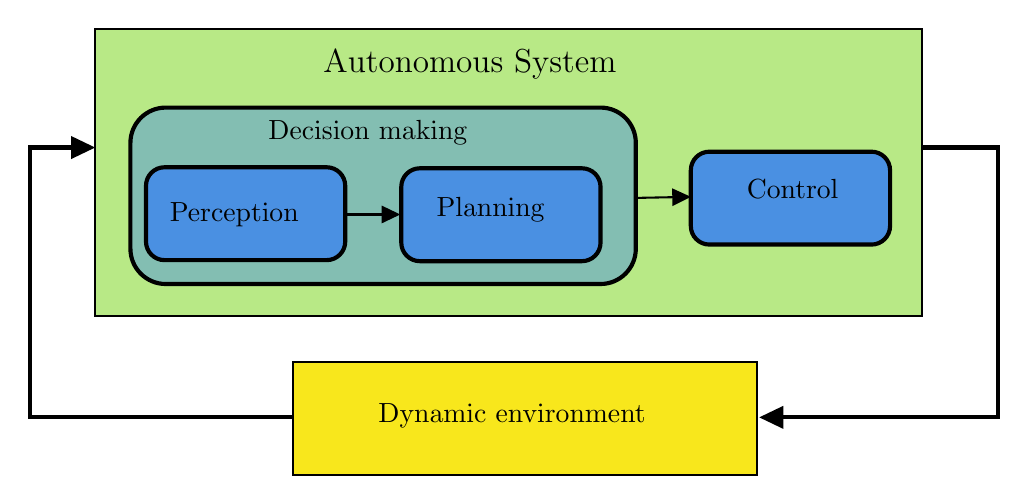
\begin{tikzpicture}[x=0.75pt,y=0.75pt,yscale=-1,xscale=1]
	%uncomment if require: \path (0,300); %set diagram left start at 0, and has height of 300
	
	%Shape: Rectangle [id:dp27957619560066704] 
	\draw  [fill={rgb, 255:red, 184; green, 233; blue, 134 }  ,fill opacity=1 ] (43,48.75) -- (441.5,48.75) -- (441.5,187.25) -- (43,187.25) -- cycle ;
	%Rounded Rect [id:dp7625981193027371] 
	\draw  [color={rgb, 255:red, 0; green, 0; blue, 0 }  ,draw opacity=1 ][fill={rgb, 255:red, 74; green, 144; blue, 226 }  ,fill opacity=1 ][line width=1.5]  (330,116.95) .. controls (330,112.01) and (334.01,108) .. (338.95,108) -- (417.05,108) .. controls (421.99,108) and (426,112.01) .. (426,116.95) -- (426,143.8) .. controls (426,148.74) and (421.99,152.75) .. (417.05,152.75) -- (338.95,152.75) .. controls (334.01,152.75) and (330,148.74) .. (330,143.8) -- cycle ;
	%Straight Lines [id:da826125804046745] 
	\draw    (304.5,130.25) -- (327,129.81) ;
	\draw [shift={(330,129.75)}, rotate = 178.88] [fill={rgb, 255:red, 0; green, 0; blue, 0 }  ][line width=0.08]  [draw opacity=0] (8.93,-4.29) -- (0,0) -- (8.93,4.29) -- cycle    ;
	%Rounded Rect [id:dp7912077043288683] 
	\draw  [color={rgb, 255:red, 0; green, 0; blue, 0 }  ,draw opacity=1 ][fill={rgb, 255:red, 74; green, 144; blue, 226 }  ,fill opacity=0.48 ][line width=1.5]  (60,103.75) .. controls (60,94.36) and (67.61,86.75) .. (77,86.75) -- (286.5,86.75) .. controls (295.89,86.75) and (303.5,94.36) .. (303.5,103.75) -- (303.5,154.75) .. controls (303.5,164.14) and (295.89,171.75) .. (286.5,171.75) -- (77,171.75) .. controls (67.61,171.75) and (60,164.14) .. (60,154.75) -- cycle ;
	%Rounded Rect [id:dp050693216378291606] 
	\draw  [color={rgb, 255:red, 0; green, 0; blue, 0 }  ,draw opacity=1 ][fill={rgb, 255:red, 74; green, 144; blue, 226 }  ,fill opacity=1 ][line width=1.5]  (67.5,124.45) .. controls (67.5,119.51) and (71.51,115.5) .. (76.45,115.5) -- (154.55,115.5) .. controls (159.49,115.5) and (163.5,119.51) .. (163.5,124.45) -- (163.5,151.3) .. controls (163.5,156.24) and (159.49,160.25) .. (154.55,160.25) -- (76.45,160.25) .. controls (71.51,160.25) and (67.5,156.24) .. (67.5,151.3) -- cycle ;
	%Rounded Rect [id:dp6167247502432494] 
	\draw  [color={rgb, 255:red, 0; green, 0; blue, 0 }  ,draw opacity=1 ][fill={rgb, 255:red, 74; green, 144; blue, 226 }  ,fill opacity=1 ][line width=1.5]  (190.5,124.95) .. controls (190.5,120.01) and (194.51,116) .. (199.45,116) -- (277.55,116) .. controls (282.49,116) and (286.5,120.01) .. (286.5,124.95) -- (286.5,151.8) .. controls (286.5,156.74) and (282.49,160.75) .. (277.55,160.75) -- (199.45,160.75) .. controls (194.51,160.75) and (190.5,156.74) .. (190.5,151.8) -- cycle ;
	%Straight Lines [id:da3281578111728798] 
	\draw    (163.5,138.25) -- (179.5,138.25) -- (187,138.25) ;
	\draw [shift={(190,138.25)}, rotate = 180] [fill={rgb, 255:red, 0; green, 0; blue, 0 }  ][line width=0.08]  [draw opacity=0] (8.93,-4.29) -- (0,0) -- (8.93,4.29) -- cycle    ;
	%Shape: Rectangle [id:dp8888738733811714] 
	\draw  [fill={rgb, 255:red, 248; green, 231; blue, 28 }  ,fill opacity=1 ] (138.5,209.25) -- (362,209.25) -- (362,263.75) -- (138.5,263.75) -- cycle ;
	
	%Straight Lines [id:da14809135342937618] 
	\draw [line width=1.5]    (442,106) -- (478,106) -- (478,236) -- (367,236) ;
	\draw [shift={(363,236)}, rotate = 360] [fill={rgb, 255:red, 0; green, 0; blue, 0 }  ][line width=0.08]  [draw opacity=0] (11.61,-5.58) -- (0,0) -- (11.61,5.58) -- cycle    ;
	%Straight Lines [id:da5537882213887542] 
	\draw [line width=1.5]    (138,236) -- (11.5,236) -- (11.5,106) -- (39,106) ;
	\draw [shift={(43,106)}, rotate = 180] [fill={rgb, 255:red, 0; green, 0; blue, 0 }  ][line width=0.08]  [draw opacity=0] (11.61,-5.58) -- (0,0) -- (11.61,5.58) -- cycle    ;
	
	% Text Node
	\draw (151.5,57.5) node [anchor=north west][inner sep=0.75pt]   [align=left] {{\large Autonomous System}};
	% Text Node
	\draw (77.5,131) node [anchor=north west][inner sep=0.75pt]   [align=left] {Perception};
	% Text Node
	\draw (206,128.5) node [anchor=north west][inner sep=0.75pt]   [align=left] {Planning};
	% Text Node
	\draw (355.5,120) node [anchor=north west][inner sep=0.75pt]   [align=left] {Control};
	% Text Node
	\draw (125,91.5) node [anchor=north west][inner sep=0.75pt]   [align=left] {Decision making};
	% Text Node
	\draw (178,228) node [anchor=north west][inner sep=0.75pt]   [align=left] {Dynamic environment};
	
	
\end{tikzpicture}
	\caption{Framework Autonomous System.}
	\label{fig:as_arch}
\end{figure}



 write it in a formal language without iusing complex words, and maintining the same number of words and concept try to uniform this text to be more readable and compact:
Perception, a fundamental aspect of \gls{av} technology, encompasses the intricate interplay between the vehicle's sensory inputs and its understanding of the surrounding environment. Through a symphony of proprioceptive, external, and exteroceptive sensors, \glspl{av} engage in a continuous dialogue with the world around them, shaping their perception of the road ahead. This perceptual framework, characterized by a diverse array of sensor technologies such as radar, cameras, LiDAR, and GPS, forms the bedrock upon which \glspl{av} navigate their operational landscapes.

The choice of sensors is a pivotal decision, with each type offering unique insights into the environment. Cameras, for instance, provide high-resolution visual data, capturing intricate details of the surroundings and facilitating robust object recognition. Radar, on the other hand, excels in detecting objects even in adverse weather conditions, offering a complementary perspective to visual data. LiDAR enhances spatial awareness, mapping out the environment with precision through laser-based technology. GPS, though not a direct sensory input, provides invaluable geospatial context, aiding in localization and route planning.

Yet, beyond the technical intricacies lies the crux of perception: how the \gls{av} interprets and synthesizes these disparate streams of sensor data into a cohesive understanding of its surroundings. Perception, in this context, is not merely the passive reception of sensory inputs but rather an active process of sense-making and contextualization. It involves discerning meaningful patterns from the sensor data, anticipating dynamic changes in the environment, and making informed decisions in real-time.

The perception systems of \glspl{av}, therefore, serve as the eyes and ears of these autonomous entities, shaping their interaction with the world and influencing their behavior on the road. It is through the lens of perception that \glspl{av} navigate complex urban environments, negotiate challenging road conditions, and ensure the safety of passengers and pedestrians alike. As technology advances and perception algorithms grow increasingly sophisticated, the future holds the promise of even greater perceptual acuity for \gls{av}, ushering in an era of safer, more efficient transportation systems.

The planning phase, as a pivotal component of the \gls{av} decision-making continuum, orchestrates a seamless transition from perception to action, synthesizing environmental cues into a cohesive course of action. At its core, this phase encapsulates a sophisticated interplay between machine intelligence and real-world dynamics, where \glspl{av} dynamically chart their trajectory amidst the ever-evolving landscape of their operational milieu.

Within this realm, the AV embarks on a deliberative journey, intricately weaving together inputs garnered from the perception phase with mission objectives and situational imperatives. Whether navigating bustling city streets, traversing expansive highways, or negotiating intricate railway networks, the \gls{av}'s planning algorithm meticulously tailors its trajectory to align with operational exigencies and safety constraints.

Moreover, the adaptability and agility inherent in the planning process imbue \glspl{av} with the capacity to respond nimbly to emergent scenarios, deftly recalibrating their path in real-time to circumvent obstacles and optimize efficiency. This dynamic recalibration, informed by a fusion of sensory inputs and predictive analytics, ensures that the AV remains resilient in the face of uncertainty, fostering a symbiotic relationship between perception and action.

It is imperative to underscore that the nuances of planning are not universal but rather bespoke to the unique characteristics of each AV archetype. Whether terrestrial, aerial, or rail-bound, the planning paradigm undergoes bespoke tailoring to harmonize with the intrinsic attributes and operational exigencies of the vehicle in question. This bespoke tailoring ensures that the planning process remains attuned to the idiosyncrasies of each domain, optimizing performance and fostering seamless integration within the broader transportation ecosystem.

In essence, the planning phase serves as the linchpin of AV autonomy, catalyzing the translation of perception into purposeful action. By orchestrating a symphony of cognitive processes and environmental awareness, this phase not only steers \glspl{av} towards their destination but also paves the way for a future where intelligent transportation systems harmoniously coalesce with the fabric of urban mobility.


Decision-making for autonomous systems involves processes through which these entities make safe and efficient decisions based on environmental information and the state of the system itself. In contexts of autonomous systems, such as \glspl{av}, decision-making is critical for safe navigation and interaction with other road users. This decision-making process encompasses a multitude of factors, including real-time sensor data, predictive analytics, and adherence to predefined rules and regulations.

Classical decision-making methods, such as rule-based systems, optimization algorithms, and probabilistic models, provide a structured approach to handling various scenarios encountered by autonomous systems. Rule-based systems rely on a set of predefined rules to guide decision-making, while optimization algorithms aim to find the best possible solution to a given problem, considering constraints and objectives. Probabilistic models, on the other hand, use statistical inference to estimate the likelihood of different outcomes, enabling decision-making under uncertainty.

In contrast, learning-based methods leverage artificial intelligence techniques to improve decision-making capabilities over time. By learning from large volumes of example data, these methods can adapt and evolve to handle complex and dynamic environments more effectively. Statistical learning techniques, such as support vector machines and decision trees, analyze patterns in data to make predictions or classifications. Deep learning algorithms, which involve neural networks with multiple layers, excel at processing complex sensory inputs, such as images or speech, to make high-level decisions. Reinforcement learning, inspired by behavioral psychology, enables autonomous systems to learn through trial and error, optimizing decisions based on feedback from the environment.

These decision-making methods play a crucial role in enabling autonomous systems to operate autonomously and safely in diverse and unpredictable environments. By combining classical and learning-based approaches, autonomous systems can navigate complex scenarios, anticipate potential hazards, and interact seamlessly with their surroundings, ultimately enhancing safety and efficiency on the road.

Within the domain of \glspl{av}, the control sub-system assumes a critical role in the precise execution of planned trajectories. Its primary function is to guide the vehicle along designated paths as determined by the planning sub-system.

A control system is tasked with regulating or maintaining process conditions within a plant to align with desired values. This is achieved by adjusting certain process variables to manipulate the variables of interest, typically the output variables. In the context of \glspl{av}, the control system is responsible for generating commands for throttle, brake, and steering inputs, which are essential for directing the vehicle's motion parameters such as position, orientation, velocity, acceleration, and jerk.

It's important to clarify that the designation of input and output variables—often referred to as manipulated/process variables and controlled variables, respectively—is with respect to the plant rather than the controller itself, a distinction that can sometimes cause confusion.

The control system plays a pivotal role within the architecture of an autonomous vehicle. As the final component of the pipeline, it assumes the responsibility for physically maneuvering the vehicle. It is the control sub-system that ultimately dictates the behavior of the ego vehicle and its interactions with the surrounding environment.

While the control sub-system relies on inputs from the perception and planning sub-systems, it is equally valid to assert that the latter two are rendered ineffective if the controller fails to accurately track the prescribed trajectory. Thus, the control sub-system not only complements but also completes the holistic framework of AV operation, ensuring seamless navigation and interaction within dynamic environments.



  
\subsection{Future Trends}

The future trends and directions of \glspl{av} are shaped by key insights from global expert discussions. The emphasis is on regulatory frameworks acting as catalysts for \gls{av} deployment, with a focus on safety, environmental impact, and societal benefits. Innovations in freight and public transport systems, such as drone delivery services and autonomous buses, are highlighted. Challenges like congestion, parking, and urban planning are acknowledged, with strategies for addressing these through technological advancements and policy adjustments. The development of common standards and data sharing protocols is vital for global adoption, alongside advancements in cybersecurity to protect emerging AV ecosystems. Overall, the future of \glspl{av} presents a complex interplay of technology, regulation, and societal acceptance, driving towards enhanced safety, efficiency, and environmental sustainability.






